\section{改进的U-Net模型设计}

% 总领起始段

\subsection{网络的改进设计}

\subsubsection{改进设计的动机}

尽管U-Net网络的跳跃连接能够有效地结合浅层和深层特征,但直接将编码器浅层特征映射与对应解码器特征级联,这种“无差别”拼接会把大量与前景无关的背景噪声一并传递,造成解码器在处理边界模糊和极小目标时,可能因为上下文信息的缺失而导致定位不准确。为了抑制冗余背景,同时保持高分辨率的边缘信息,本研究提出了改进的U-Net模型设计,在每一级跳跃通路中引入注意力门,依据编码器高层语义对编码器特征进行动态像素级筛选。

注意力机制的核心思想是通过动态地调整特征图的权重,自动聚焦于目标区域,抑制无关背景的干扰。这种方法能够增强模型对重要区域的敏感度,提高模型对小目标的定位能力\cite{oktay2018}。具体而言,注意力门根据输入特征图和从粗尺度上提取的上下文信息,计算每个像素的注意力系数,并利用该系数对特征图进行加权,从而只保留对分割任务有用的区域。这一策略无需额外的外部局部化模型,通过自动学习重要区域,有效提升了模型的分割精度,同时避免了传统多阶段模型中冗余计算和参数过多的问题。

%在网络结构中的嵌入位置上,注意力模块被集成到U-Net的跳跃连接部分。传统的U-Net通过将编码器的低层特征图与解码器高层特征图进行拼接来进行信息传递,而在引入注意力机制后,注意力模块被放置在编码器和解码器跳跃连接的中间。在这一位置,注意力模块可以根据解码器的上下文信息来加权编码器的特征图,确保网络关注到最重要的区域并忽略无关背景。具体而言,在每个跳跃连接处,编码器的特征图 $x_l$ 和解码器的特征图 $g_l$ 会被送入注意力门模块,经过加权后再与解码器的上采样特征进行拼接。这一设计使得注意力机制能够在局部区域进行动态学习,从而提高了分割的精度,尤其是在分割小目标和复杂背景时的表现。

\subsubsection{注意力门模块的结构与原理}

%此外,注意力模块采用的网格注意力机制(Grid Attention Mechanism),相较于传统通道注意力(如SENet)仅关注通道维度,本研究的网格注意力机制通过局部区域的动态调整,兼顾空间与通道信息,更适用于医学图像中目标形态多变的场景。

注意力门模块的内部结构主要由三个关键部分组成:输入特征的加权过程、注意力系数的计算以及门控机制的输出。具体而言,该模块包括权重矩阵 $W_x$ 和 $W_g$、非线性激活函数 ReLU、Sigmoid 激活函数以及注意力权重的计算等组成部分。

首先,注意力门模块接收来自U-Net编码器的特征图 $x_l$ 和解码器的门控信号 $g_l$ 作为输入。$x_l$ 为编码器第 $l$ 层输出的特征图,$g_l$ 则是来自解码器的特征图,它为后续的注意力加权提供上下文信息。为了将这两者的特征进行融合,模块采用了两种1×1卷积操作:一个用于处理编码器的特征图 $x_l$,另一个用于处理解码器的门控信号 $g_l$。这两者都通过对应的卷积核 $W_x$ 和 $W_g$ 进行映射到一个中间空间,从而保持信息的一致性并准备后续的注意力计算。

接下来,在这两路特征图被处理后,它们通过ReLU激活函数进行非线性转换,这一步骤有助于引入非线性特征表达,使得网络能够更好地学习到复杂的关系。此时,经过ReLU激活的特征图被送入一个加法操作,进行特征融合,得到一个结合了编码器和解码器信息的中间表示。为了进一步处理该表示并生成最终的注意力权重,模块通过Sigmoid激活函数计算得到一个归一化的注意力系数 $\alpha_l$,该系数决定了每个像素的权重。最后,这些权重通过逐元素相乘的方式与编码器特征图 $x_l$ 进行加权,从而生成加权后的特征图 $\tilde{x}_l = \alpha_l \cdot x_l$。

在计算过程中,注意力系数 $\alpha_l$ 的计算公式如下:

\begin{equation}
    q_{\text{att}}^l = \psi^T \left( \sigma_1 (W_x^T x_l + W_g^T g_l + b_g) \right) + b_\psi
\end{equation}

\begin{equation}
    \alpha_l = \sigma_2 \left( q_{\text{att}}^l(x_l, g_l; \Theta_{\text{att}}) \right)
\end{equation}

其中,$\sigma_1$ 和 $\sigma_2$ 分别为 ReLU 和 Sigmoid 激活函数,$W_x$ 和 $W_g$ 是用于特征映射的权重矩阵,$\psi$ 是线性变换矩阵,$b_g$ 和 $b_\psi$ 是偏置项。在这个公式中,$q_{\text{att}}^l$ 是通过加法操作和线性变换后得到的注意力得分,$\alpha_l$ 是最终计算得到的注意力系数。通过Sigmoid激活,$\alpha_l$ 的值范围被限制在$[0, 1]$之间,能够根据不同位置的特征重要性动态调整每个位置的注意力权重。

为了进一步探究注意力门的机制和作用,本文直观展示了同一张 ISIC 图像分别在原始 U-Net 与 Attention-U-Net 四级跳跃通路上的特征图,并截取其中 4 个通道进行并排可视化,如图 \ref{fig:skip_vs_gate_vis} 所示。图中左半四列(Skip:ch0-ch3)对应原始U-Net网络的编码器跳跃连接后准备和解码器拼接的特征图;右半四列(Gate:ch0-ch3)则是 Attention U-Net经过注意力门调制后的准备和解码器拼接的特征图。纵向从上到下依次为四级跳跃连接(Skip1/Gate1-Skip4/Gate4)。

\begin{figure}[!htbp]
    \centering
    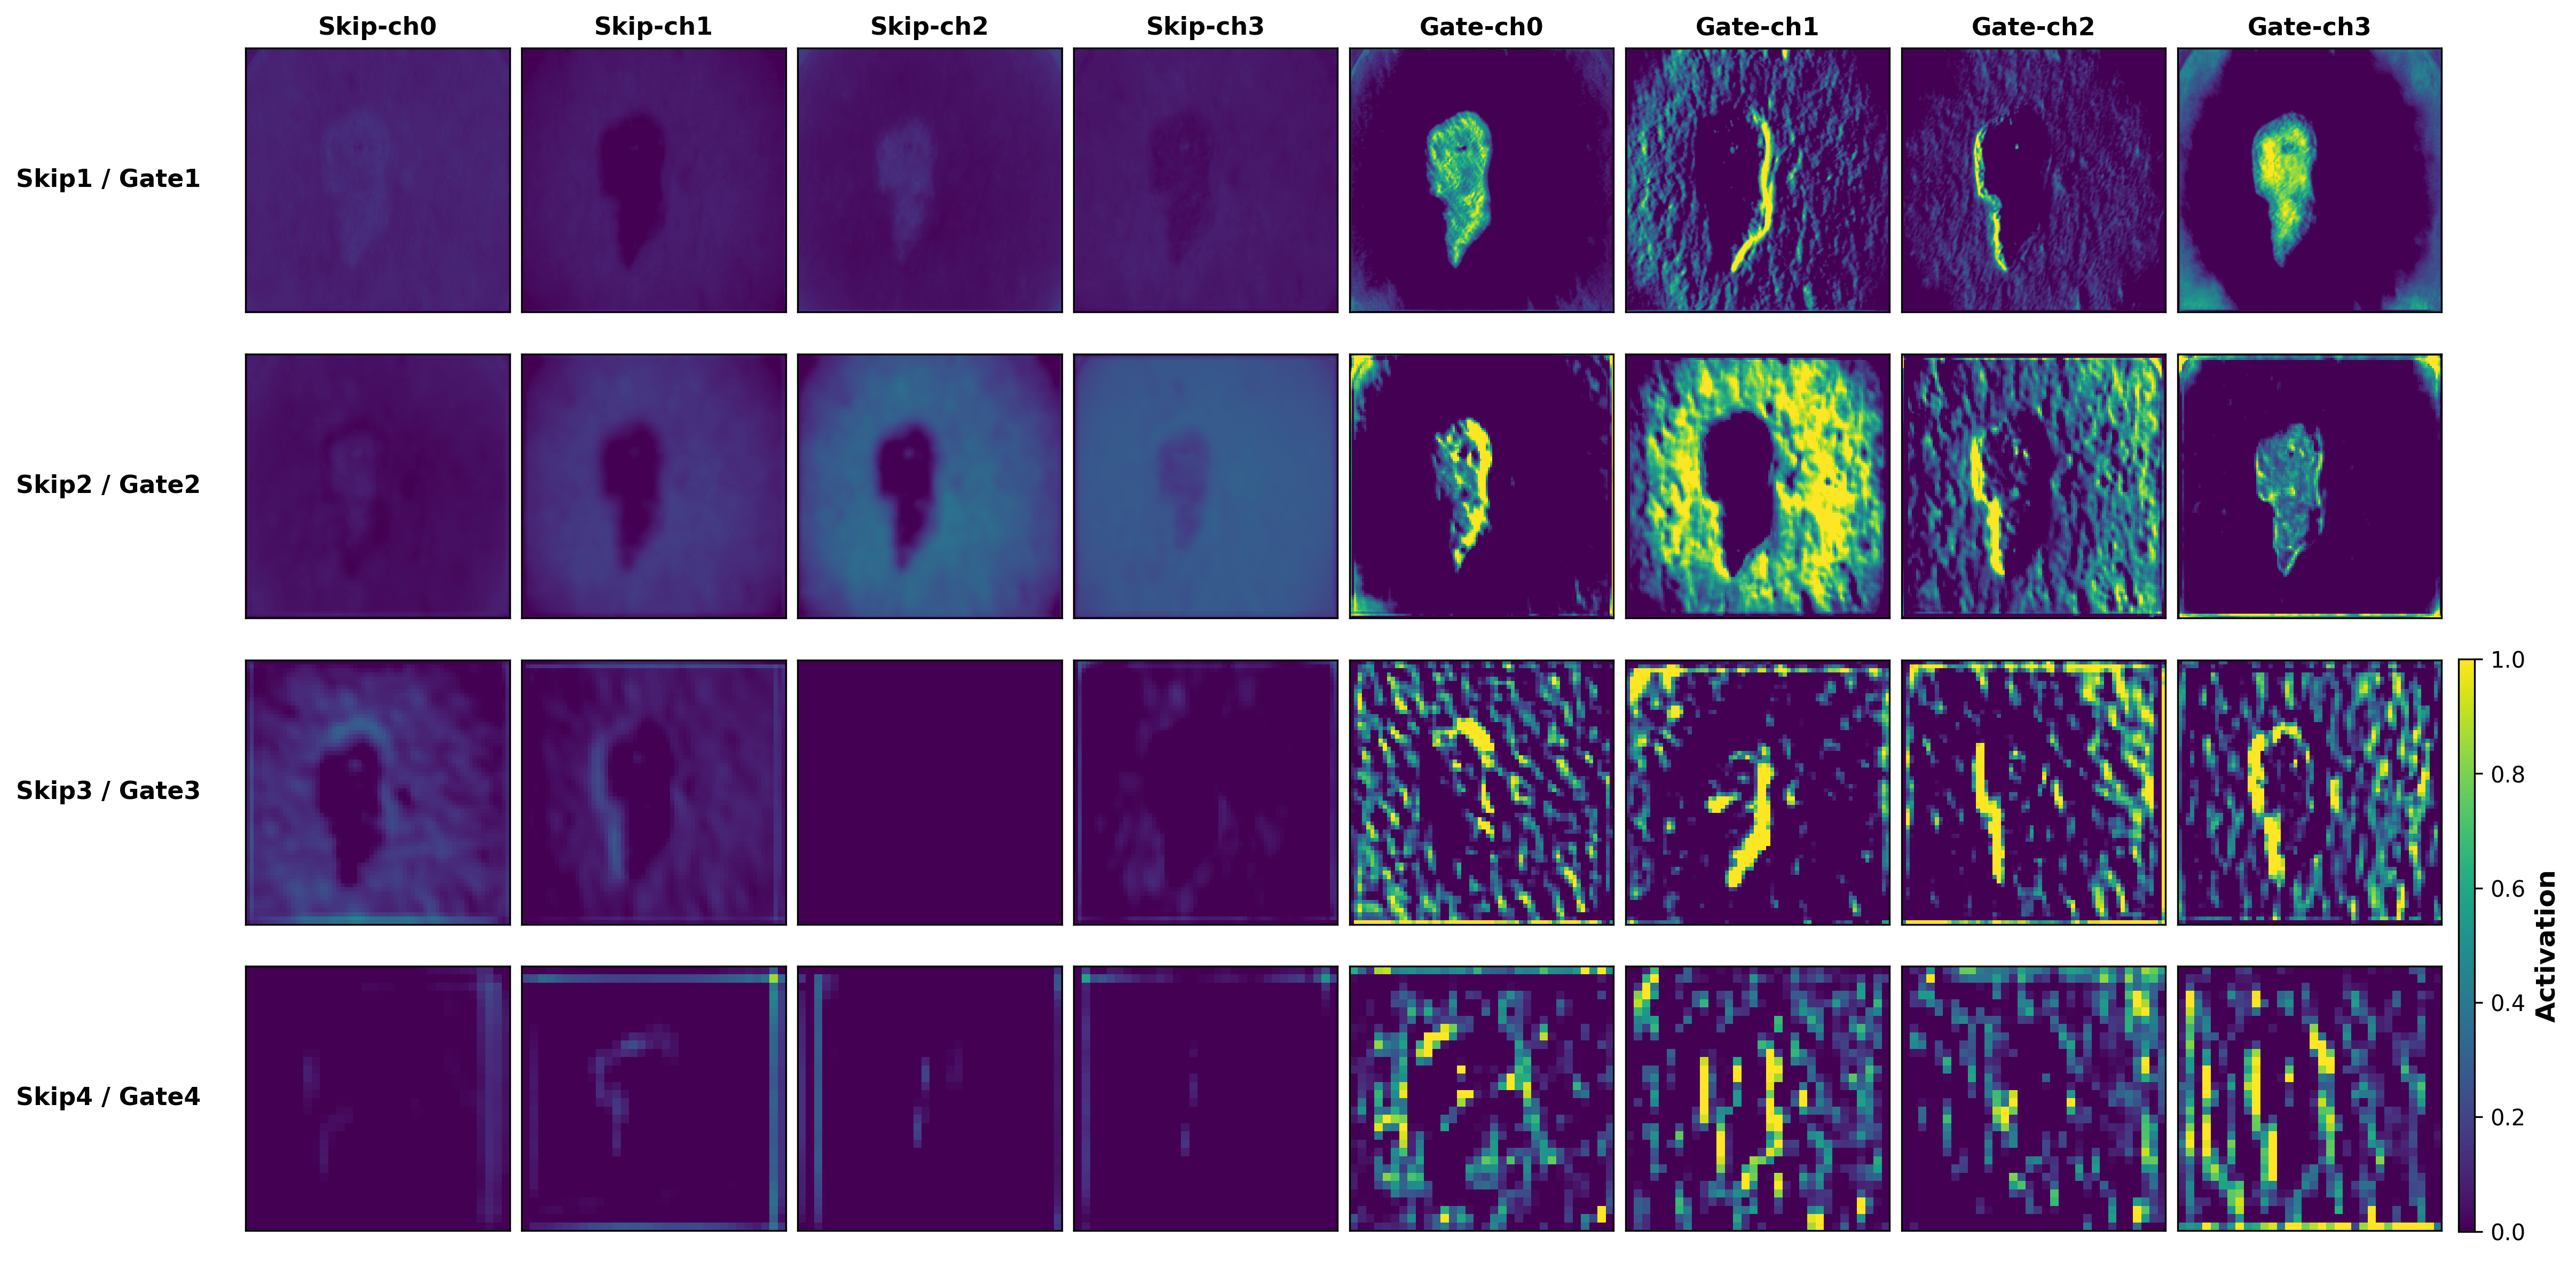
\includegraphics[width=\textwidth]{fig/unet_vs_attunet_feature_compare.png}
    \caption{}
    \label{fig:skip_vs_gate_vis}
\end{figure}

通过对比,可以得到三点关键观察:

\begin{enumerate}
    \item 浅层抑噪:在 Skip1 与 Skip2 中,原始特征几乎整幅图像均有弱激活,背景纹理与病灶边界难以区分;而 Gate1、Gate2 中大量背景像素被压制至 0 – 0.2 的低激活区,仅在病灶主体及其边缘保留显著响应,说明注意力门已在最早层面过滤掉无用纹理。
    
    \item 深层聚焦:随着网络加深(Skip3、Skip4),原始跳跃特征仍夹杂噪声条纹,而 Gate3、Gate4 的高亮区域收缩并对齐于病灶外轮廓,形成清晰的连贯带;由此可见,门控权重不仅抑制背景,还在深层强化对判别性边界的响应。
    
    \item 信息重加权而非简单剪裁:Gate-ch 通道在病灶区域的激活强度显著高于 Skip-ch(色条 0.6 – 1.0),而非单纯“置零”背景后保持原强度。这表明注意力门起到了增益—抑制双向调制 的作用:一方面降低噪声,另一方面放大关键特征,从而在解码阶段提供更清晰的边界信息。
\end{enumerate}

上述可视化与前文对注意力门工作机制的理论分析一致,也为后续消融实验(见第 4.2 节)将呈现的定量改进提供直观佐证:在加入注意力门后,我们将看到验证集 Recall 和 Dice 均显著提高,而 Precision 仅出现轻微波动。这说明注意力门能够在跳跃连接中对高分辨率特征进行“像素级甄别”,在最大限度保留判别性信息的同时,有效压制背景噪声,从源头减少漏检而不过度引入误检。

\subsection{损失函数的改进设计}

在损失函数的设计上,改进的U-Net模型采用Dice Loss和Cross-Entropy Loss的混合损失函数,即以相等权重线性叠加Dice损失与像素级交叉熵(CE)损失,以充分兼顾类别不平衡下的区域重叠度优化与梯度稳定性。设网络输出的类别概率图(像素总数为$N$)为:$ P=\left\{p_{i}\right\}_{i=1}^{N} $,真实分割掩膜为$ G=\left\{g_{i}\right\}_{i=1}^{N} $,其中$ p_{i} \in[0,1], g_{i} \in\{0,1\}$分别是像素$i$的前景概率和真实标签。则:

\begin{equation}
    \mathcal{L}_{\text {Dice }}=1-\frac{2 \sum_{i=1}^{N} p_{i} g_{i}}{\sum_{i=1}^{N} p_{i}+\sum_{i=1}^{N} g_{i}+\varepsilon}
\end{equation}

\begin{equation}
    \mathcal{L}_{\mathrm{CE}}=-\frac{1}{N} \sum_{i=1}^{N}\left[g_{i} \ln \left(p_{i}\right)+\left(1-g_{i}\right) \ln \left(1-p_{i}\right)\right]
\end{equation}

\begin{equation}
    \mathcal{L}_{\text {mix }}=0.5 \mathcal{L}_{\text {Dice }}+0.5 \mathcal{L}_{\mathrm{CE}}
\end{equation}

其中$ \varepsilon=10^{-6} $用于数值平滑以防零分母。Dice项直接对预测与标注的重叠区域进行归一化度量,能在小体积病灶场景下显著提升召回;交叉熵项则提供像素级对数似然的密集监督,改善早期训练阶段梯度稀疏、收敛震荡等问题。

\subsection{训练策略的改进设计}

在工程设计上,本研究引入注意力机制改进的U-Net进行了若干关键实现选择,以提高计算效率和模型的泛化能力。首先,在U-Net的解码器中,我们选择使用双线性插值代替转置卷积进行上采样。双线性插值是一种常见的图像插值方法,它通过对相邻像素进行加权平均来生成上采样后的图像,这样可以有效避免转置卷积中可能出现的伪影问题,并且计算开销较小。

此外,网络中的BatchNorm(批归一化)操作并未在所有层次中都加入,而是根据需要灵活使用。批归一化通过对每一层的输入进行标准化处理,能够加速网络的收敛并减小过拟合的风险。在改进的U-Net中,BatchNorm的使用主要集中在卷积层之后的部分,以保证特征图的稳定性并加速训练过程。